\section{Methodology}\label{sec:methods}

Previous studies have demonstrated the feasibility of 
holistic HPC I/O analysis and used it to observe anomalous I/O behavior and
contributing factors over short time scales~\cite{Lockwood2017}. This methodology was later formalized in the specification of the \tokio (\tokiolong) framework~\cite{Lockwood2018tokio}. 
In this work, we use 
the \tokio framework
%a similar methodology 
to collect 
%and analyze 
a complete
year of I/O metrics on multiple production platforms. We analyze the collected data to observe transient and long-term trends in I/O performance variability.  This section
summarizes the \tokio framework, 
describes the production HPC platforms that we have 
%deployed it on, 
used in this study,
and introduces our methodology for active probing of storage system
performance.

\subsection{Data collection framework}\label{sec:methods/tokio}

%A holistic approach to understanding I/O behavior is a necessity given the move towards more complicated I/O architectures (in terms of number of constituent components, like high-level I/O libraries, I/O middleware systems, and low-level storage hardware) on these systems. \tokio's primary goal is to arm system users, administrators, and I/O researchers with the necessary tools to navigate this complexity and to make meaningful observations into how workloads interact with the I/O subsystem.

\begin{figure}
    \centering
    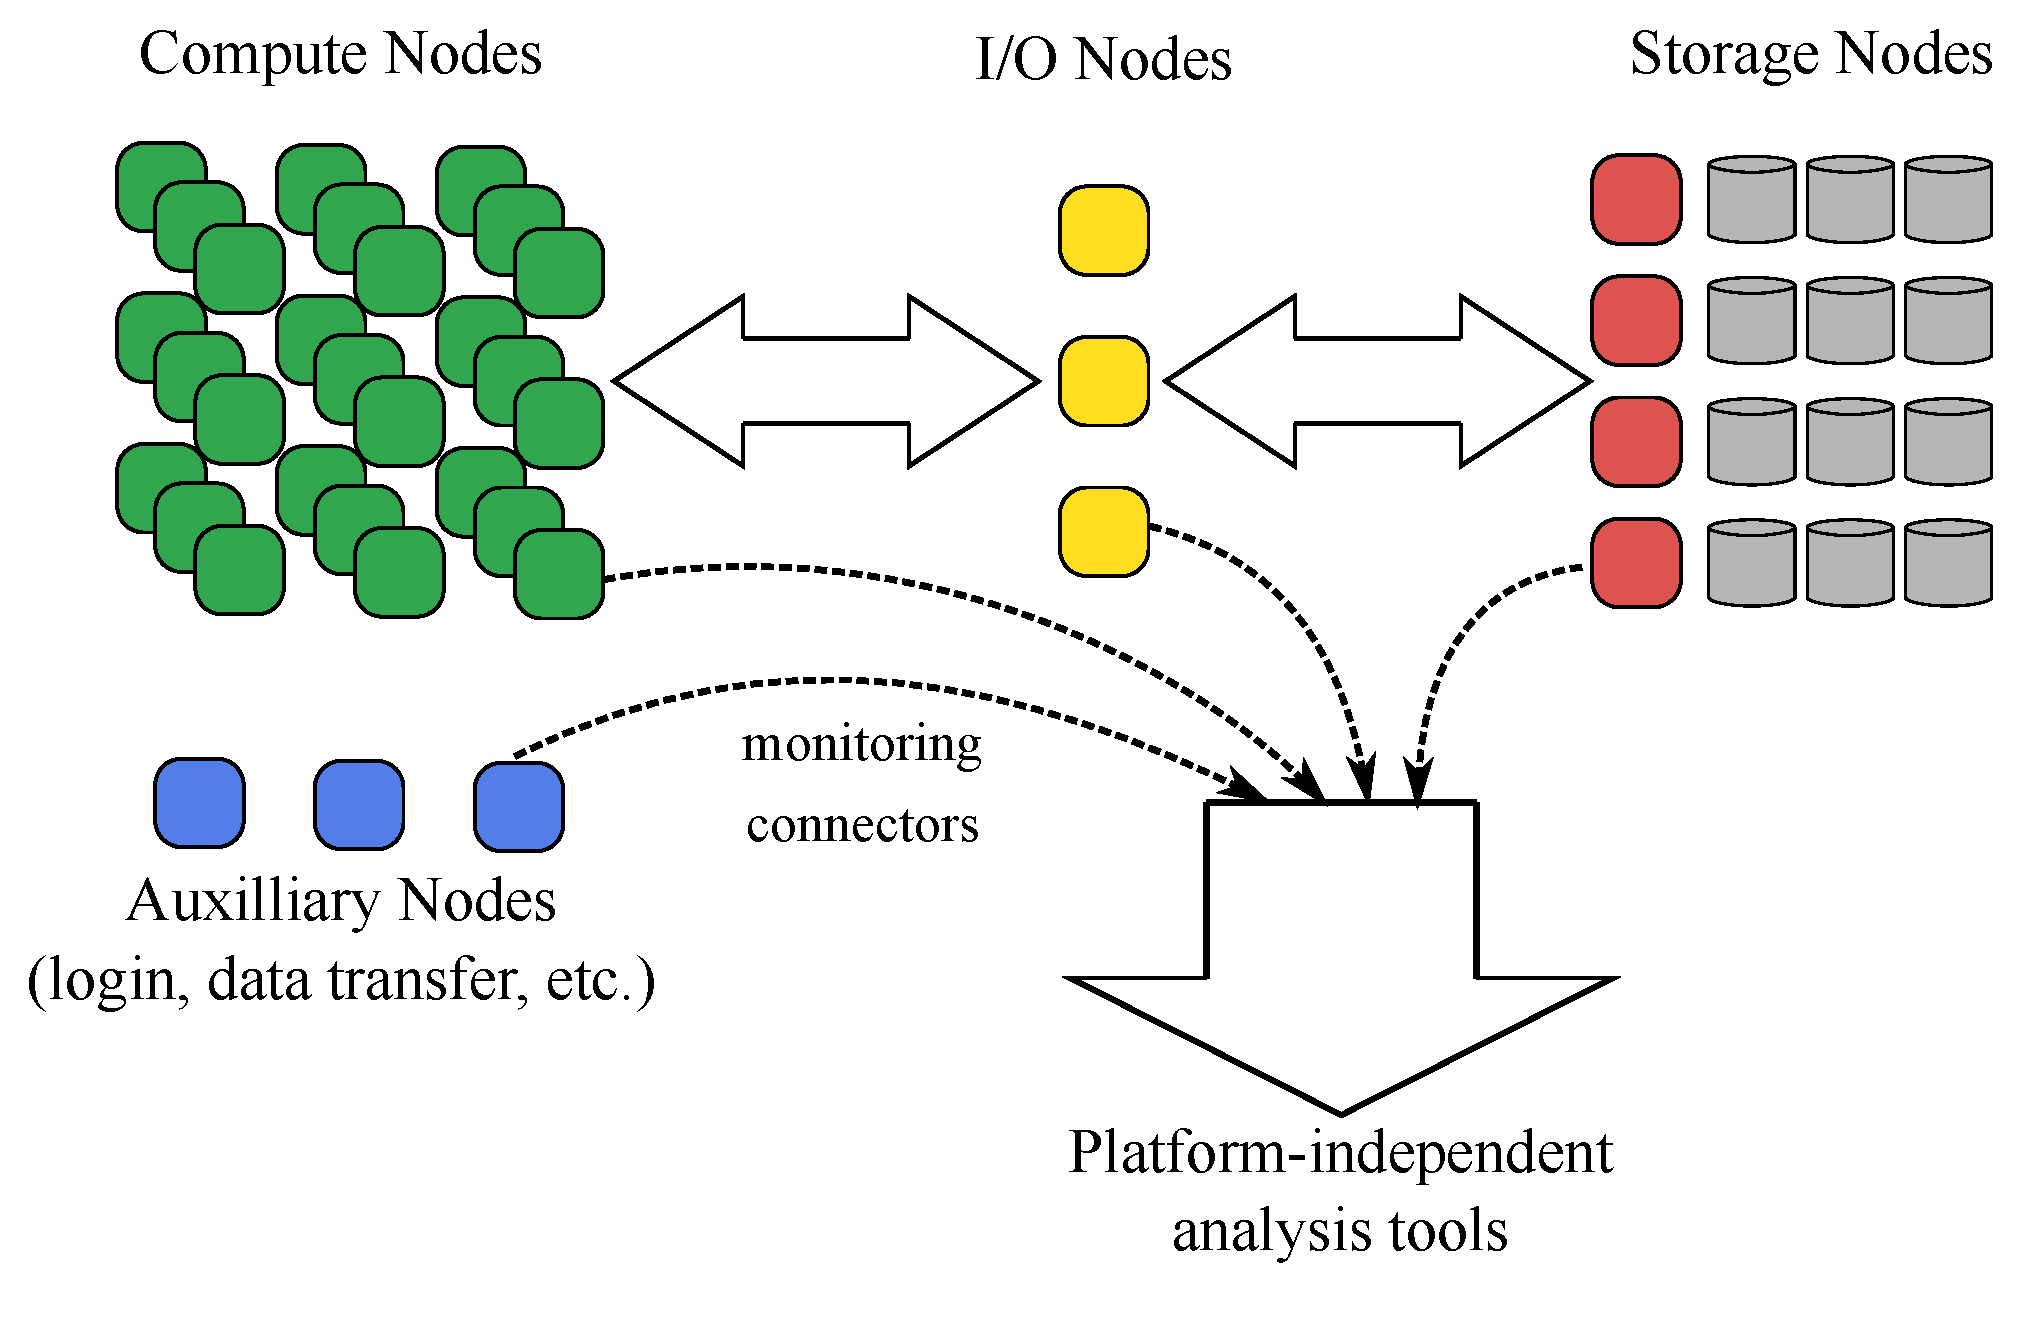
\includegraphics[width=0.9\columnwidth]{tokio}
        \vspace{-.1in}
    \caption{Overview of the \tokio framework, providing holistic analysis across the numerous components of the I/O subsystem on HPC platforms.}
    \label{fig:tokio-framework}
\end{figure}

\tokio is a framework facilitating holistic characterization and analysis of I/O workloads running on today's production HPC systems. Conceptually, it provides an abstraction layer between component-level monitoring tools already deployed on HPC platforms and higher-level I/O analysis tools that utilize this data, as illustrated in  Figure~\ref{fig:tokio-framework}. The fundamental roles of the \tokio framework are to collate monitoring data from distinct components, integrate and normalize the data from these components, and present coherent interfaces for indexing and accessing this data.

\tokio uses a modularized software architecture and a generic data format
specification for system monitoring data, simplifying portability to new HPC
platforms. Software modularity is accomplished by defining abstract
\textit{connectors} to monitoring sources; these connectors then expose interfaces for
extracting relevant data in a format suitable for \tokio.  A generic
timeseries format is used for semantically consistent access to data
originating from distinct monitoring tools, even though each tool uses its
own underlying data format with its own scope and granularity.
The timeseries data format designates a number of metrics
that are common to classes of monitoring components.  For example, file system
monitoring tools often gather common metrics such as read/write bandwidths
and operation counts. \tokio connectors can convert the native data formats
of their underlying tools to this generic format in-memory as part of
on-demand analysis, or \tokio-aware tools can archive directly into this
format on-disk. These design decisions greatly simplify the process of
integrating new monitoring sources as well the process of developing
platform-independent I/O analysis tools.  This study in particular relies on
integrated analysis of the following monitoring connectors:

\begin{itemize}[leftmargin=*]
\item \textbf{Application-level monitoring}: \textit{Darshan}~\cite{Carns2009} is an application I/O characterization tool that is commonly deployed at production HPC facilities. It provides a condensed set of I/O counters, timers, and other statistics for each file accessed by a given application.

\item \textbf{File system workload monitoring}: \textit{LMT}~\cite{lmt} and \textit{ggiostat}~\cite{Lockwood2017} are examples of 
file system monitoring tools for Lustre and GPFS deployments, respectively. These tools each capture metrics quantifying file system workloads periodically over a given time interval, with some of these metrics being common to both tools (e.g., observed read/write bandwidths, number of specific metadata operations issued, etc.) and other metrics being file system specific (e.g., the CPU utilization on a given Lustre metadata server captured by LMT).

\item \textbf{File system capacity/health monitoring}: File system specific tools like Lustre's \textit{lfs} and \textit{lctl} or GPFS's \textit{mmdf} and \textit{mmlsdisk} can be invoked periodically to capture current file system state, including the capacity and failover status of individual storage servers and/or disks in the system.

\item \textbf{Resource manager monitoring}: Resource managers like Slurm~\cite{2003slurm} often keep a detailed accounting of all jobs that execute on a particular system, including useful details like the size of the job and its placement across available compute nodes.
\end{itemize}

The telemetric data from these connectors are aggregated into \emph{attributes} associated with each job, and all of the attributes associated with a job are represented as \emph{feature vectors}.
Wherever possible, attributes are also expressed as \emph{coverage factors}~\cite{Lockwood2017} which quantify the fraction of system-wide activity that can be attributed to the job of interest.
For example, a job's \emph{bandwidth coverage factor} is the number of bytes read and written by that job's application (measured by Darshan) divided by the number of bytes read and written across the entire parallel file system (measured by LMT or ggiostat) while that job was running.
A coverage factor of 1.0 indicates that a job was the exclusive consumer of
a resource, while a coverage factor of 0.4 indicates that other competing
jobs consumed 60\% of the total delivered resources.

%Each job in this study typically produces a feature vector with 220 attributes including derived values.
% gkl: above is misleading because all feature vectors are the same size, but they may have different attributes left undefined.
Each job in this study produced a feature vector with 220 attributes; 96 attributes come from application-level monitoring, 101 come from file system workload monitoring, 21 come from file system health monitoring, 6 come from resource manager monitoring, and the remainder are job-wide metadata.
The exact number of attributes defined in each
%The exact size of the 
feature vector depends on what connectors are available on the target platform at the time the job is executed.

\subsection{Platforms}\label{sec:methods/platforms}

% Please add the following required packages to your document preamble:
% \usepackage{multirow}
\begin{table}
\centering
\caption{Description of \nersc and \alcf test platforms.}
\label{tab:platform-descriptions}
\begin{tabular}{|c|c|c|c|c|}
\hline
                                                                                   & \textbf{Platform}                                                              & \textbf{FS Name (Type)} & \textbf{Size} & \textbf{Peak Rate}     \\ \hline
\multirow{3}{*}{\textbf{\begin{tabular}[c]{@{}c@{}}\edison\\ (\nersc)\end{tabular}}} & \multirow{3}{*}{\begin{tabular}[c]{@{}c@{}}Cray XC30\\ 5,586 CNs\end{tabular}} & \scratchone (Lustre)               & 2.2 PiB       & 48 GB/sec              \\ \cline{3-5} 
                                                                                   &                                                                                & \scratchtwo (Lustre)               & 2.2 PiB       & 48 GB/sec              \\ \cline{3-5} 
                                                                                   &                                                                                & \scratchthree (Lustre)               & 3.3 PiB       & 72 GB/sec              \\ \hline
\textbf{\begin{tabular}[c]{@{}c@{}}\cori\\ (\nersc)\end{tabular}}                    & \begin{tabular}[c]{@{}c@{}}Cray XC40\\ 12,076 CNs\end{tabular}                 & \cscratch (Lustre)               & 28 PiB      & 744 GB/sec \\ \hline
\textbf{\begin{tabular}[c]{@{}c@{}}\mira\\ (\alcf)\end{tabular}}                     & \begin{tabular}[c]{@{}c@{}}IBM BG/Q\\ 49,152 CNs\end{tabular}                  & \mirafsone (GPFS)               & 7.0 PiB       & 90 GB/sec              \\ \hline
\end{tabular}
\end{table}

We applied the \tokio framework on the \edison and \cori systems at \nersc and the \mira system at the \alcf. Each of these platforms, along with their corresponding file systems analyzed as part of this study, are briefly described in Table~\ref{tab:platform-descriptions}.

Darshan is installed and automatically enabled on each of these systems, transparently characterizing the I/O workloads of a large portion of  each system's job population. 
\nersc has deployed LMT for full-time monitoring of the Lustre scratch
volumes on both \edison and \cori, while the \alcf has deployed ggiostat to
do the same for the GPFS volumes on \mira.
\nersc systems additionally utilize the Slurm resource manager, which allows for the capture of detailed metadata for every job executed on \edison or \cori.
\tokio uses these data sources in-place to provide a unified holistic view
of I/O performance without copying data to a dedicated database facility.

\subsection{I/O Performance Probes}\label{sec:methods/benchmarks}

\begin{table}
\centering
\caption{I/O Performance Probe Motifs}
\label{my-label}
\begin{tabular}{|r|c|c|}
\hline
\multicolumn{1}{|l|}{}    & \begin{tabular}[c]{@{}c@{}}$O(10^1 \textup{ MiB})$\\\textbf{Transfers}\end{tabular} & \begin{tabular}[c]{@{}c@{}}$O(10^2 \textup{ MiB})$\\\textbf{Transfers}\end{tabular} \\ \hline
\textbf{Shared File}      & IOR/shared                 & VPIC and BDCATS              \\ \hline
\textbf{File Per Process} & IOR/fpp                    & HACC                         \\ \hline
\end{tabular}
\label{tab:benchmark-motifs}
\end{table}

To measure the performance variation on the systems described in Section \ref{sec:methods/platforms}, we ran four I/O-intensive application benchmarks on a daily basis from February 14, 2017 to February 15, 2018.
We utilize these benchmarking runs as another monitoring source for this
study, actively probing the user-perceived I/O performance of each analyzed file system on a daily basis across a range of representative I/O motifs.
The four underlying benchmarks (VPIC, BDCATS, HACC, and IOR) were chosen to exercise a variety of I/O workloads and covered the four I/O motifs listed in Table \ref{tab:benchmark-motifs} in both read and write modes.
Each probe was configured to run identically to previous work~\cite{Lockwood2017} with the goal of using a substantial fraction of the I/O subsystem's peak bandwidth while using minimal production cycles.

All probes ran using 256 nodes (4,096 processes) on \cori, 128 nodes (2,048 processes) on \edison, and 1,024 nodes (16,384 processes) on \mira.
Data was striped as widely as possible in all cases; this corresponds to
striping over every OST (for \cori and \edison) or every LUN (for \mira).
In the case of \cori and \edison, each job had access to the full I/O bandwidth of its I/O nodes as well, but due to the way in which I/O nodes are allocated in a fixed ratio to job size on Blue Gene/Q systems, \mira jobs were restricted to the bandwidth provided by eight I/O nodes.

81.9\% of the intended probes successfully generated results, providing 
11,986 performance observations across \mira, \cori, and \edison over the
course of a year.
The remaining 18.1\% of potential probes failed due to system downtime, malfunctions of component-level monitoring tools or the automated test scheduling, queue wait times that exceeded 24 hours, or using excessive walltime.


%\TODO{Add details of the number of processes the benchmarks ran with, and how the file systems are set up, i.e., number of OSTs on \cori, number of I/O nodes used on \mira 
%\\
%\edison was mentioned in the previous paragraph; Figure 1 doesn't have the results. -- Suren}
% DONE - 2018-03-26 gkl
